% Model report generated by SolverMapp.
% Compile with pdflatex (twice, for the equation and algorithm references).
\documentclass[11pt,a4paper]{article}
\usepackage[T1]{fontenc}
\usepackage[utf8]{inputenc}
\usepackage{lmodern}
\usepackage{amsmath,amssymb}
\usepackage{booktabs,longtable}
\usepackage{siunitx}
\usepackage{algorithm}
\usepackage{algpseudocode}
\usepackage{tikz}
\usetikzlibrary{positioning,shapes.geometric,shapes.misc,arrows.meta}
\usepackage{adjustbox}
\usepackage[hidelinks]{hyperref}

\title{Vectors and matrices: linear system, products, vector ODE, vector root}
\author{}
\date{\today}

\begin{document}
\maketitle

The model consists of 10 equations in 17 variables: 7 inputs, 1 state variable, 2 intermediate variables and 7 outputs. It is solved in 2 steps (Algorithm~\ref{alg:solution}).

\section{Nomenclature}
\begin{longtable}{@{}l p{0.48\linewidth} l l@{}}
  \toprule
  Symbol & Description & Unit & Value \\
  \midrule
  \endhead
  \bottomrule
  \endfoot
  \multicolumn{4}{@{}l}{\textit{Inputs}} \\
  $\mathbf{K}$ & Stiffness & \si{N/m} & 4, -1; -1, 3 \\
  $\mathbf{F}$ & Load & \si{N} & 1, 2 \\
  $\mathbf{a}$ & a & \si{m} & 1, 2, 3 \\
  $\mathbf{b}$ & b & \si{m} & 4, 5, 6 \\
  $\mathbf{M}$ & Rotation & \si{1/s} & 0, 1; -1, 0 \\
  $t$ & Time & \si{s} & \num{0} \\
  $\mathbf{c}$ & Squares & -- & 4, 9 \\
  \addlinespace
  \multicolumn{4}{@{}l}{\textit{State variables}} \\
  $\mathbf{y}$ & State & -- & 1, 0 \\
  \addlinespace
  \multicolumn{4}{@{}l}{\textit{Intermediate variables}} \\
  $\mathbf{u}$ & Displacement & \si{m} &  \\
  $\mathbf{r}$ & Same, by inverse & \si{m} &  \\
  \addlinespace
  \multicolumn{4}{@{}l}{\textit{Outputs}} \\
  $E$ & Energy & \si{J} &  \\
  $\mathbf{w}$ & a x b & \si{m^{2}} &  \\
  $s$ & a . b & \si{m^{2}} &  \\
  $n_a$ & |a| & \si{m} &  \\
  $\mathbf{z}$ & Unknown & -- &  \\
  $\mathbf{P}$ & K K\textasciicircum{}T & \si{N^{2}/m^{2}} &  \\
  $\mathbf{q}$ & 2r + u & \si{m} &  \\
\end{longtable}

\section{Governing equations}

\subsection{Stiffness system}
\begin{equation}
  \mathbf{K}\mathbf{u} = \mathbf{F}
  \label{eq:stiffness-system}
\end{equation}
\noindent where

\noindent\begin{tabular}{@{\quad}l@{\quad}p{0.7\linewidth}@{}}
  $\mathbf{u}$ & Displacement, \si{m} \\
  $\mathbf{K}$ & Stiffness, \si{N/m} \\
  $\mathbf{F}$ & Load, \si{N} \\
\end{tabular}

\noindent Linear in $\mathbf{u}$: solved directly as a linear system (Gaussian elimination with partial pivoting).

\subsection{Inverse solve}
\begin{equation}
  \mathbf{r} = \mathbf{K}^{-1}\mathbf{F}
  \label{eq:inverse-solve}
\end{equation}
\noindent where

\noindent\begin{tabular}{@{\quad}l@{\quad}p{0.7\linewidth}@{}}
  $\mathbf{r}$ & Same, by inverse, \si{m} \\
  $\mathbf{K}$ & Stiffness, \si{N/m} \\
  $\mathbf{F}$ & Load, \si{N} \\
\end{tabular}


\subsection{Cross product}
\begin{equation}
  \mathbf{w} = \mathbf{a} \times \mathbf{b}
  \label{eq:cross-product}
\end{equation}
\noindent where

\noindent\begin{tabular}{@{\quad}l@{\quad}p{0.7\linewidth}@{}}
  $\mathbf{w}$ & a x b, \si{m^{2}} \\
  $\mathbf{a}$ & a, \si{m} \\
  $\mathbf{b}$ & b, \si{m} \\
\end{tabular}


\subsection{Dot product}
\begin{equation}
  s = \mathbf{a} \cdot \mathbf{b}
  \label{eq:dot-product}
\end{equation}
\noindent where

\noindent\begin{tabular}{@{\quad}l@{\quad}p{0.7\linewidth}@{}}
  $s$ & a . b, \si{m^{2}} \\
  $\mathbf{a}$ & a, \si{m} \\
  $\mathbf{b}$ & b, \si{m} \\
\end{tabular}


\subsection{Norm}
\begin{equation}
  n_a = \|\mathbf{a}\|
  \label{eq:norm}
\end{equation}
\noindent where

\noindent\begin{tabular}{@{\quad}l@{\quad}p{0.7\linewidth}@{}}
  $n_a$ & |a|, \si{m} \\
  $\mathbf{a}$ & a, \si{m} \\
\end{tabular}


\subsection{Rotation ODE}
\begin{equation}
  \frac{d\mathbf{y}}{dt} = \mathbf{M}\mathbf{y}
  \label{eq:rotation-ode}
\end{equation}
\noindent where

\noindent\begin{tabular}{@{\quad}l@{\quad}p{0.7\linewidth}@{}}
  $\mathbf{y}$ & State, dimensionless \\
  $\mathbf{M}$ & Rotation, \si{1/s} \\
  $t$ & Time, \si{s} \\
\end{tabular}

\noindent Integrated over $t$ from $0$ to $1$ with the classical fourth-order Runge–Kutta method in 50 steps, starting from the start value of $\mathbf{y}$.

\subsection{Nonlinear vector root}
\begin{equation}
  \mathbf{z} \odot \mathbf{z} = \mathbf{c}
  \label{eq:nonlinear-vector-root}
\end{equation}
\noindent where

\noindent\begin{tabular}{@{\quad}l@{\quad}p{0.7\linewidth}@{}}
  $\mathbf{z}$ & Unknown, dimensionless \\
  $\mathbf{c}$ & Squares, dimensionless \\
\end{tabular}

\noindent Implicit in $\mathbf{z}$: solved for the root of the residual (left side minus right side) by Newton–Raphson iteration from the start value of $\mathbf{z}$, until the relative step is below \num{1e-12}, with at most 50 iterations.

\subsection{Gram matrix}
\begin{equation}
  \mathbf{P} = \mathbf{K}\mathbf{K}^T
  \label{eq:gram-matrix}
\end{equation}
\noindent where

\noindent\begin{tabular}{@{\quad}l@{\quad}p{0.7\linewidth}@{}}
  $\mathbf{P}$ & K K\textasciicircum{}T, \si{N^{2}/m^{2}} \\
  $\mathbf{K}$ & Stiffness, \si{N/m} \\
\end{tabular}


\subsection{Strain energy}
\begin{equation}
  E = \frac{1}{2}\mathbf{u}^T\mathbf{K}\mathbf{u}
  \label{eq:strain-energy}
\end{equation}
\noindent where

\noindent\begin{tabular}{@{\quad}l@{\quad}p{0.7\linewidth}@{}}
  $E$ & Energy, \si{J} \\
  $\mathbf{u}$ & Displacement, \si{m} \\
  $\mathbf{K}$ & Stiffness, \si{N/m} \\
\end{tabular}


\subsection{Combination}
\begin{equation}
  \mathbf{q} = 2 \mathbf{r} + \mathbf{u}
  \label{eq:combination}
\end{equation}
\noindent where

\noindent\begin{tabular}{@{\quad}l@{\quad}p{0.7\linewidth}@{}}
  $\mathbf{q}$ & 2r + u, \si{m} \\
  $\mathbf{r}$ & Same, by inverse, \si{m} \\
  $\mathbf{u}$ & Displacement, \si{m} \\
\end{tabular}


\section{Solution algorithm}
\begin{algorithm}[htbp]
  \caption{Solution procedure}\label{alg:solution}
  \begin{algorithmic}[1]
    \State Set the inputs $\mathbf{K}$, $\mathbf{F}$, $\mathbf{a}$, $\mathbf{b}$, $\mathbf{M}$ and $\mathbf{c}$
    \State Set the start values $\mathbf{y}$
    \State Solve the linear system Eq.~\eqref{eq:stiffness-system} for $\mathbf{u}$
    \State Compute $\mathbf{r}$ from Eq.~\eqref{eq:inverse-solve}
    \State Compute $\mathbf{w}$ from Eq.~\eqref{eq:cross-product}
    \State Compute $s$ from Eq.~\eqref{eq:dot-product}
    \State Compute $n_a$ from Eq.~\eqref{eq:norm}
    \For{$t = 0$ to $1$ in 50 steps} \Comment{RK4}
      \State Advance $\mathbf{y}$ by one RK4 step of Eq.~\eqref{eq:rotation-ode}
    \EndFor
    \State Start from the start value of $\mathbf{z}$
    \Repeat \Comment{Newton–Raphson}
      \State $\mathbf{z} \leftarrow \mathbf{z} - R(\mathbf{z}) / R'(\mathbf{z})$, with $R$ the residual of Eq.~\eqref{eq:nonlinear-vector-root}
    \Until{the relative step in $\mathbf{z}$ is below \num{1e-12} (at most 50 iterations)}
    \State Compute $\mathbf{P}$ from Eq.~\eqref{eq:gram-matrix}
    \State Compute $E$ from Eq.~\eqref{eq:strain-energy}
    \State Compute $\mathbf{q}$ from Eq.~\eqref{eq:combination}
  \end{algorithmic}
\end{algorithm}

Figure~\ref{fig:flowchart} shows the same procedure as a flowchart.

\begin{figure}[htbp]
  \centering
  \begin{adjustbox}{max width=\linewidth, max totalheight=0.9\textheight}
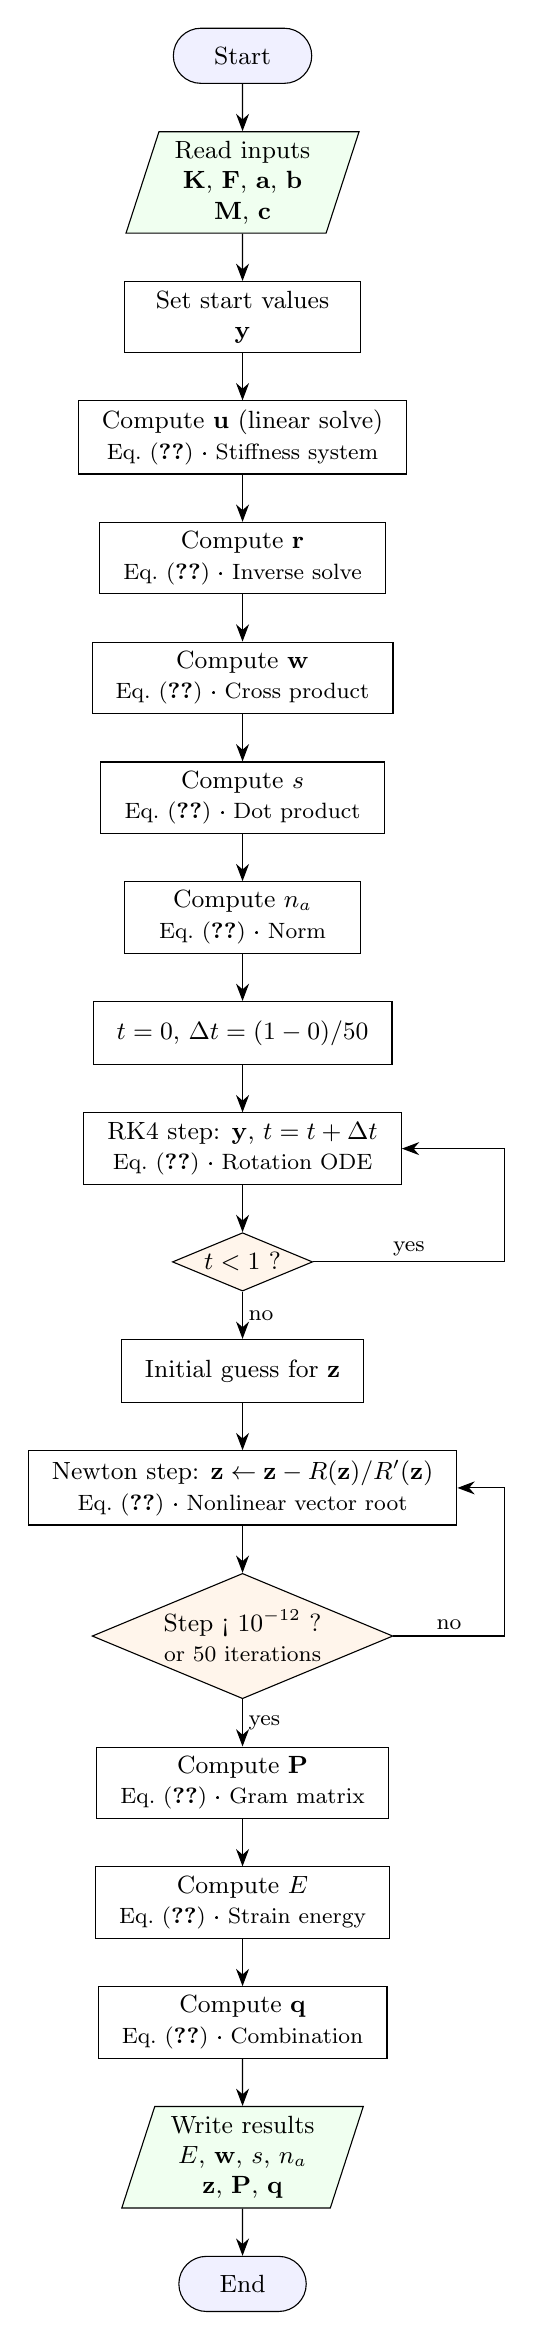
\begin{tikzpicture}[
  node distance=6mm, >={Stealth[length=2.2mm]}, font=\small,
  every node/.style={align=center},
  term/.style={draw, rounded rectangle, minimum height=7mm, inner xsep=5mm, fill=blue!6},
  io/.style={draw, trapezium, trapezium left angle=72, trapezium right angle=108, trapezium stretches body, minimum height=8mm, inner xsep=2mm, fill=green!6},
  proc/.style={draw, rectangle, minimum height=8mm, minimum width=30mm, inner xsep=3mm},
  dec/.style={draw, diamond, aspect=2.4, inner sep=1pt, fill=orange!8},
  lbl/.style={font=\footnotesize, inner sep=2pt}]
  \node[term] (n1) {Start};
  \node[io, below=of n1] (n2) {Read inputs \\ $\mathbf{K}$, $\mathbf{F}$, $\mathbf{a}$, $\mathbf{b}$ \\ $\mathbf{M}$, $\mathbf{c}$};
  \node[proc, below=of n2] (n3) {Set start values \\ $\mathbf{y}$};
  \node[proc, below=of n3] (n4) {Compute $\mathbf{u}$ (linear solve) \\ {\footnotesize Eq.~\eqref{eq:stiffness-system} \textperiodcentered{} Stiffness system}};
  \node[proc, below=of n4] (n5) {Compute $\mathbf{r}$ \\ {\footnotesize Eq.~\eqref{eq:inverse-solve} \textperiodcentered{} Inverse solve}};
  \node[proc, below=of n5] (n6) {Compute $\mathbf{w}$ \\ {\footnotesize Eq.~\eqref{eq:cross-product} \textperiodcentered{} Cross product}};
  \node[proc, below=of n6] (n7) {Compute $s$ \\ {\footnotesize Eq.~\eqref{eq:dot-product} \textperiodcentered{} Dot product}};
  \node[proc, below=of n7] (n8) {Compute $n_a$ \\ {\footnotesize Eq.~\eqref{eq:norm} \textperiodcentered{} Norm}};
  \node[proc, below=of n8] (n9) {$t = 0$, $\Delta t = (1 - 0) / 50$};
  \node[proc, below=of n9] (n10) {RK4 step: $\mathbf{y}$, $t = t + \Delta t$ \\ {\footnotesize Eq.~\eqref{eq:rotation-ode} \textperiodcentered{} Rotation ODE}};
  \node[dec, below=of n10] (n11) {$t < 1$ ?};
  \node[proc, below=of n11] (n12) {Initial guess for $\mathbf{z}$};
  \node[proc, below=of n12] (n13) {Newton step: $\mathbf{z} \leftarrow \mathbf{z} - R(\mathbf{z}) / R'(\mathbf{z})$ \\ {\footnotesize Eq.~\eqref{eq:nonlinear-vector-root} \textperiodcentered{} Nonlinear vector root}};
  \node[dec, below=of n13] (n14) {Step < $10^{-12}$ ? \\ {\footnotesize or 50 iterations}};
  \node[proc, below=of n14] (n15) {Compute $\mathbf{P}$ \\ {\footnotesize Eq.~\eqref{eq:gram-matrix} \textperiodcentered{} Gram matrix}};
  \node[proc, below=of n15] (n16) {Compute $E$ \\ {\footnotesize Eq.~\eqref{eq:strain-energy} \textperiodcentered{} Strain energy}};
  \node[proc, below=of n16] (n17) {Compute $\mathbf{q}$ \\ {\footnotesize Eq.~\eqref{eq:combination} \textperiodcentered{} Combination}};
  \node[io, below=of n17] (n18) {Write results \\ $E$, $\mathbf{w}$, $s$, $n_a$ \\ $\mathbf{z}$, $\mathbf{P}$, $\mathbf{q}$};
  \node[term, below=of n18] (n19) {End};
  \coordinate (E) at (current bounding box.east);
  \coordinate (L0) at ([xshift=6mm]E);
  \draw[->] (n1) -- (n2);
  \draw[->] (n2) -- (n3);
  \draw[->] (n3) -- (n4);
  \draw[->] (n4) -- (n5);
  \draw[->] (n5) -- (n6);
  \draw[->] (n6) -- (n7);
  \draw[->] (n7) -- (n8);
  \draw[->] (n8) -- (n9);
  \draw[->] (n9) -- (n10);
  \draw[->] (n10) -- (n11);
  \draw[->] (n11) -- node[lbl, right] {no} (n12);
  \draw[->] (n12) -- (n13);
  \draw[->] (n13) -- (n14);
  \draw[->] (n14) -- node[lbl, right] {yes} (n15);
  \draw[->] (n15) -- (n16);
  \draw[->] (n16) -- (n17);
  \draw[->] (n17) -- (n18);
  \draw[->] (n18) -- (n19);
  \draw[->] (n11.east) -- node[lbl, above] {yes} (n11.east -| L0) |- (n10.east);
  \draw[->] (n14.east) -- node[lbl, above] {no} (n14.east -| L0) |- (n13.east);
\end{tikzpicture}
  \end{adjustbox}
  \caption{Flowchart of the solution procedure}\label{fig:flowchart}
\end{figure}

\end{document}